En 2025, el mercado de tarjetas madre presenta una variedad de modelos avanzados que ofrecen compatibilidad con las últimas tecnologías y procesadores. A continuación, se destacan algunos de los modelos más actuales y recomendados:

\subsection{MSI MAG B850 Tomahawk MAX WiFi}

Esta placa base es reconocida por su excelente relación calidad-precio, ofreciendo Wi-Fi 7, Ethernet de 5GbE y dos ranuras PCIe 5.0 por aproximadamente \$230 \cite{tomshardware2025}.

\begin{figure}[H]
  \centering
  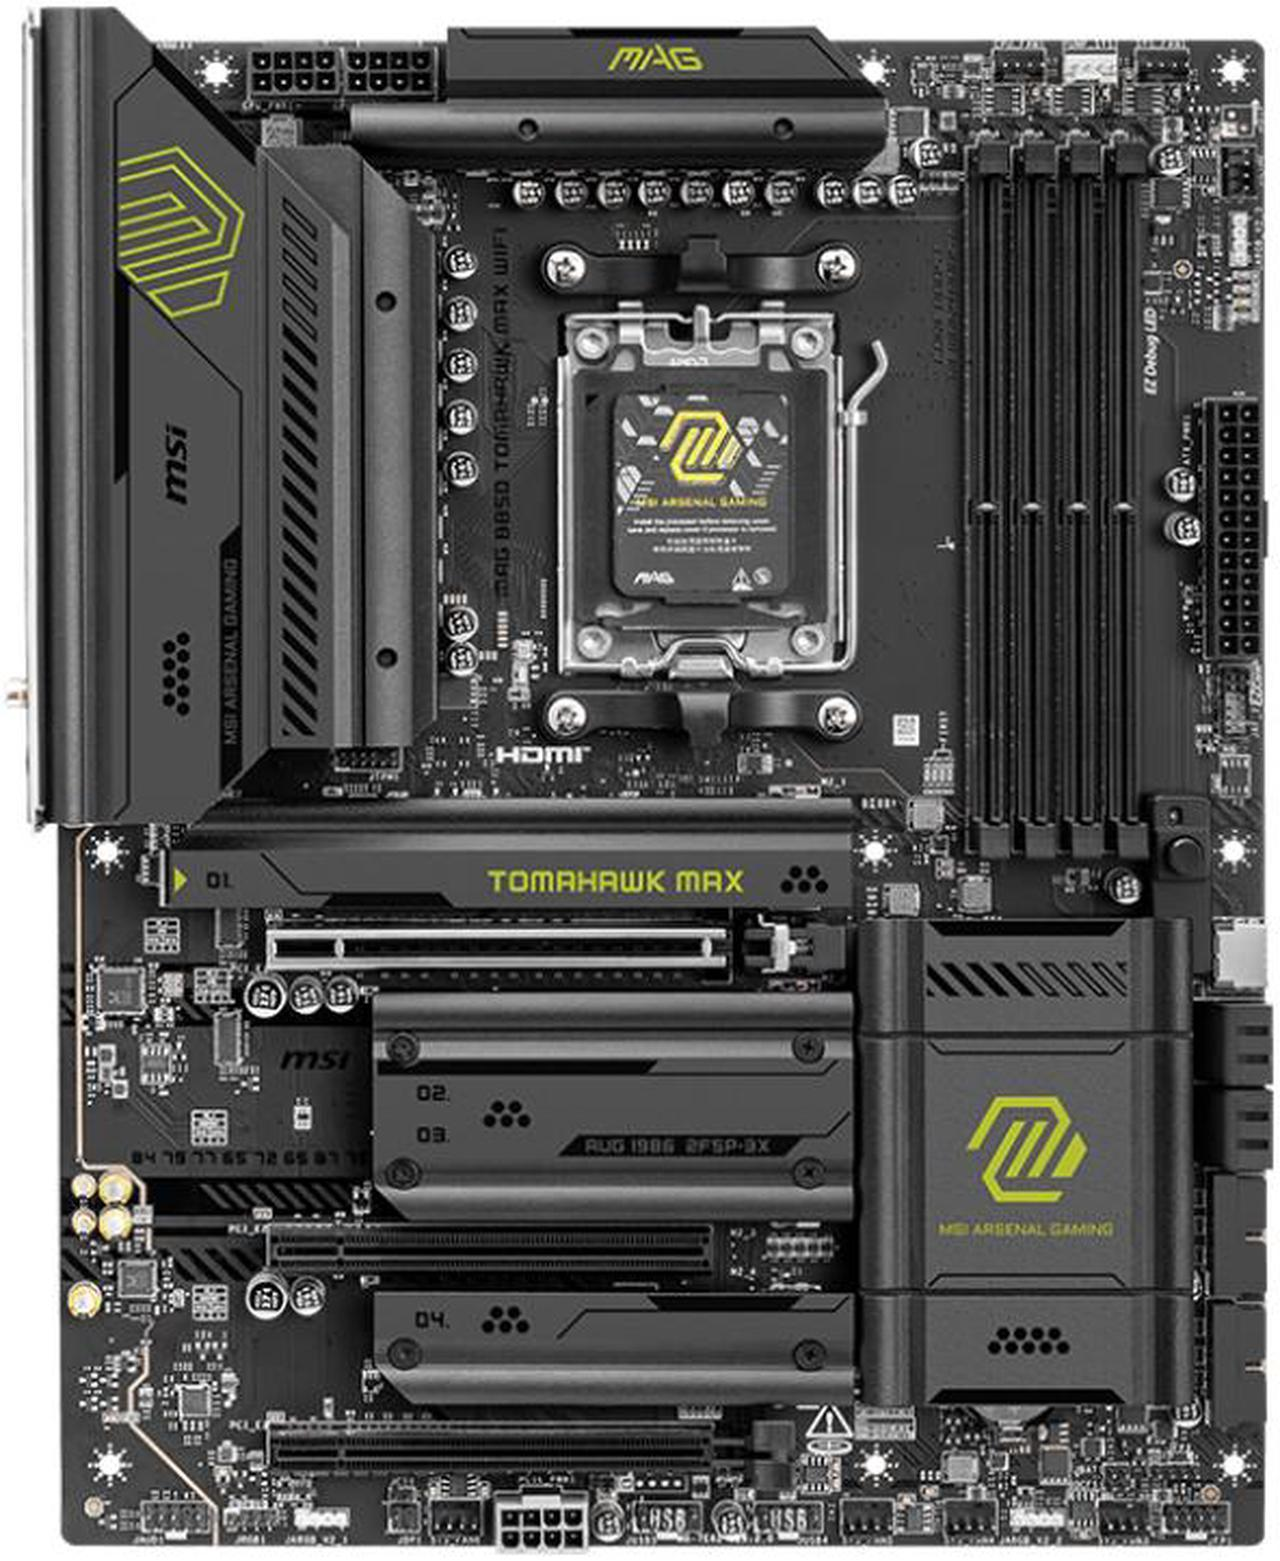
\includegraphics[scale=0.1]{imagenes/tomahawk.png}
  \caption{MSI MAG B850 Tomahawk MAX WiFi}
\end{figure}

\subsection{ASUS ROG Strix B550-F Gaming}

Ideal para entusiastas de la informática, esta placa base combina rendimiento y estabilidad, incorporando un protector de E/S preinstalado, BIOS Flashback y SafeSlot. Además, ofrece una red Intel Ethernet de 2.5 Gbps con ASUS LANGuard para conexiones rápidas y seguras\cite{lavanguardiaB550F}.

\begin{figure}[H]
  \centering
  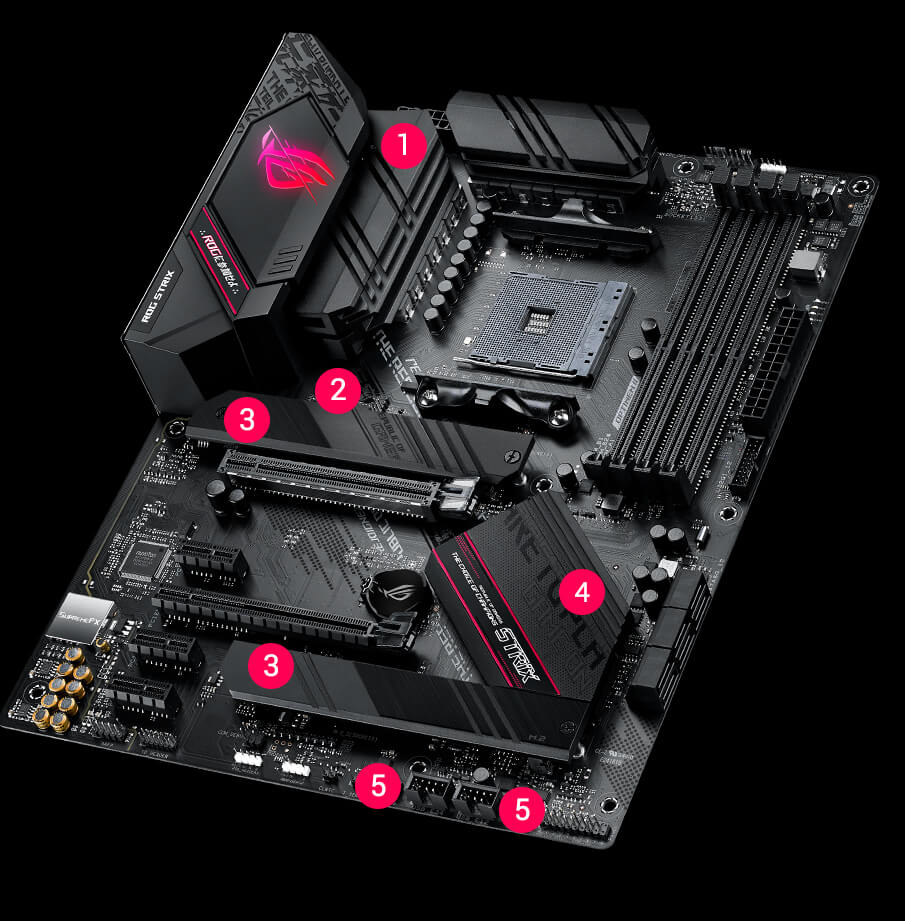
\includegraphics[scale=0.1]{imagenes/strix.png}
  \caption{ASUS ROG Strix B550-F Gaming}
\end{figure}

\subsection{ASUS TUF Gaming B550M-PLUS WiFi II}

Destaca por su compatibilidad con una amplia gama de procesadores AMD Ryzen. Con componentes TUF y Digi+ VRM, garantiza una vida útil prolongada. Su diseño centrado en la refrigeración y conectividad la convierte en una opción favorita entre los gamers \cite{lavanguardiaTUF}.

\begin{figure}[H]
  \centering
  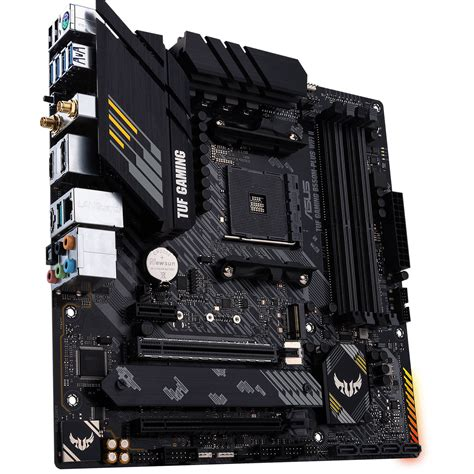
\includegraphics[scale=0.2]{imagenes/asusb550.png}
  \caption{ASUS TUF Gaming B550M-PLUS WiFi II}
\end{figure}

\subsection{ASUS TUF Gaming Z890-Pro Wi-Fi}

Diseñada para gamers, esta tarjeta madre facilita la instalación y soporta procesadores Intel Core Ultra 200 series. Ofrece cuatro ranuras de memoria DDR5 DIMM de hasta 192GB, cinco ranuras de expansión PCIe y cuatro ranuras M.2 con disipadores dedicados. Además, cuenta con LAN 2.5G, Wi-Fi 7 y múltiples puertos USB de alta velocidad \cite{asustufz890}.

\begin{figure}[H]
  \centering
  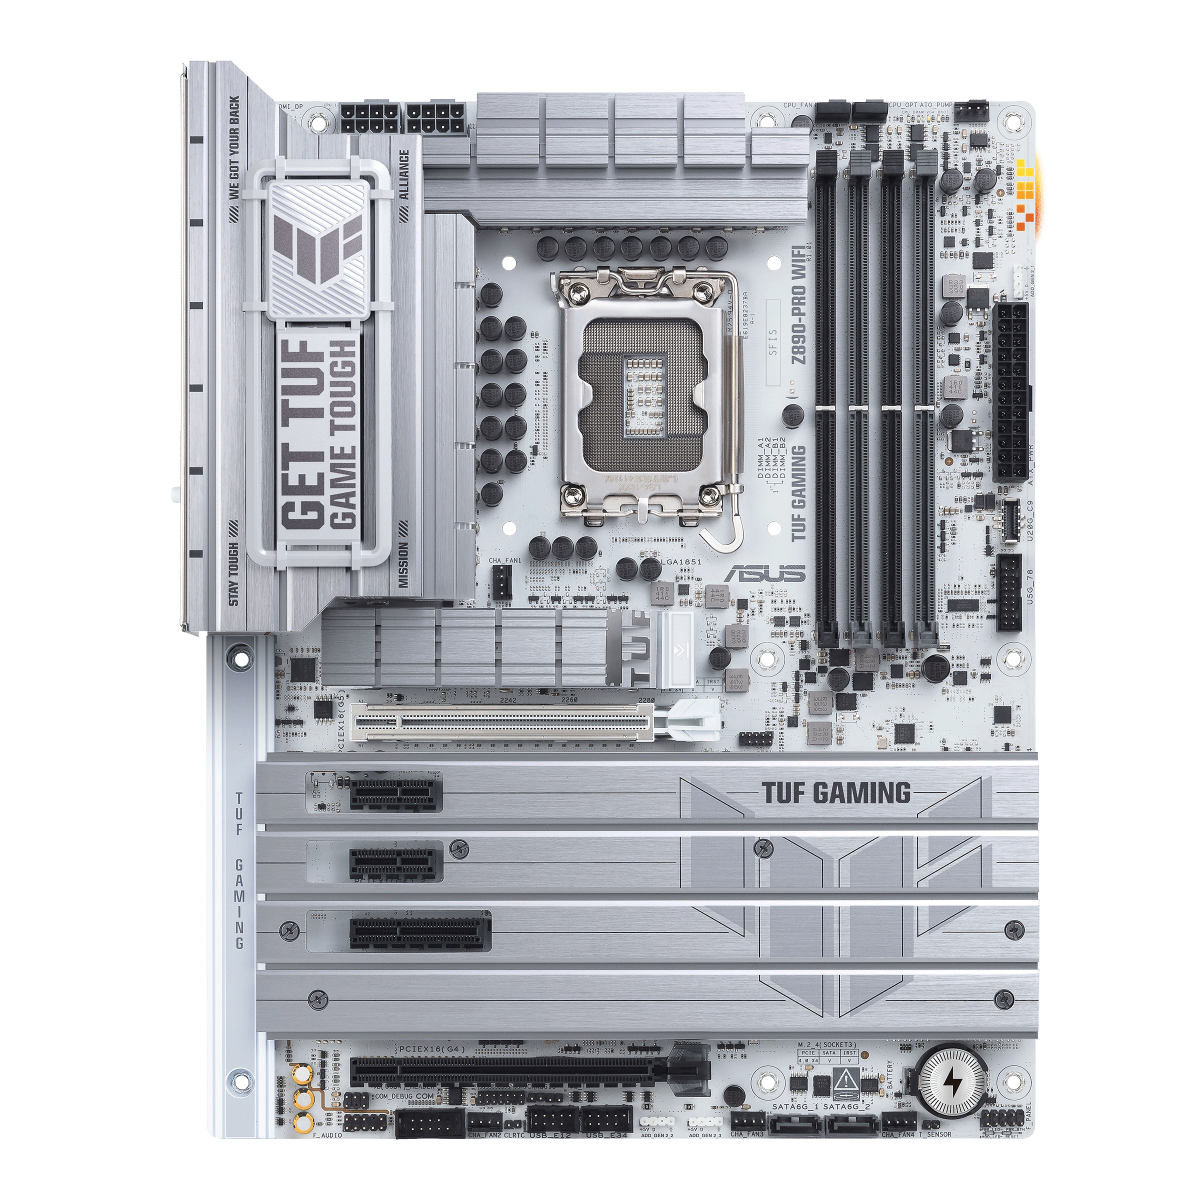
\includegraphics[scale=0.2]{imagenes/asusz890.png}
  \caption{ASUS TUF Gaming Z890-Pro Wi-Fi}
\end{figure}

\subsection{MSI MAG Z890 TOMAHAWK WIFI}

Esta tarjeta madre ATX está preparada para las próximas generaciones de procesadores y la inteligencia artificial. Cuenta con el chipset Intel Z890, soporte para hasta 256 GB de memoria DDR5, múltiples opciones de almacenamiento y conectividad avanzada, incluyendo 5G LAN y Wi-Fi 7 \cite{msiz890tomahawk}.

\begin{figure}[H]
  \centering
  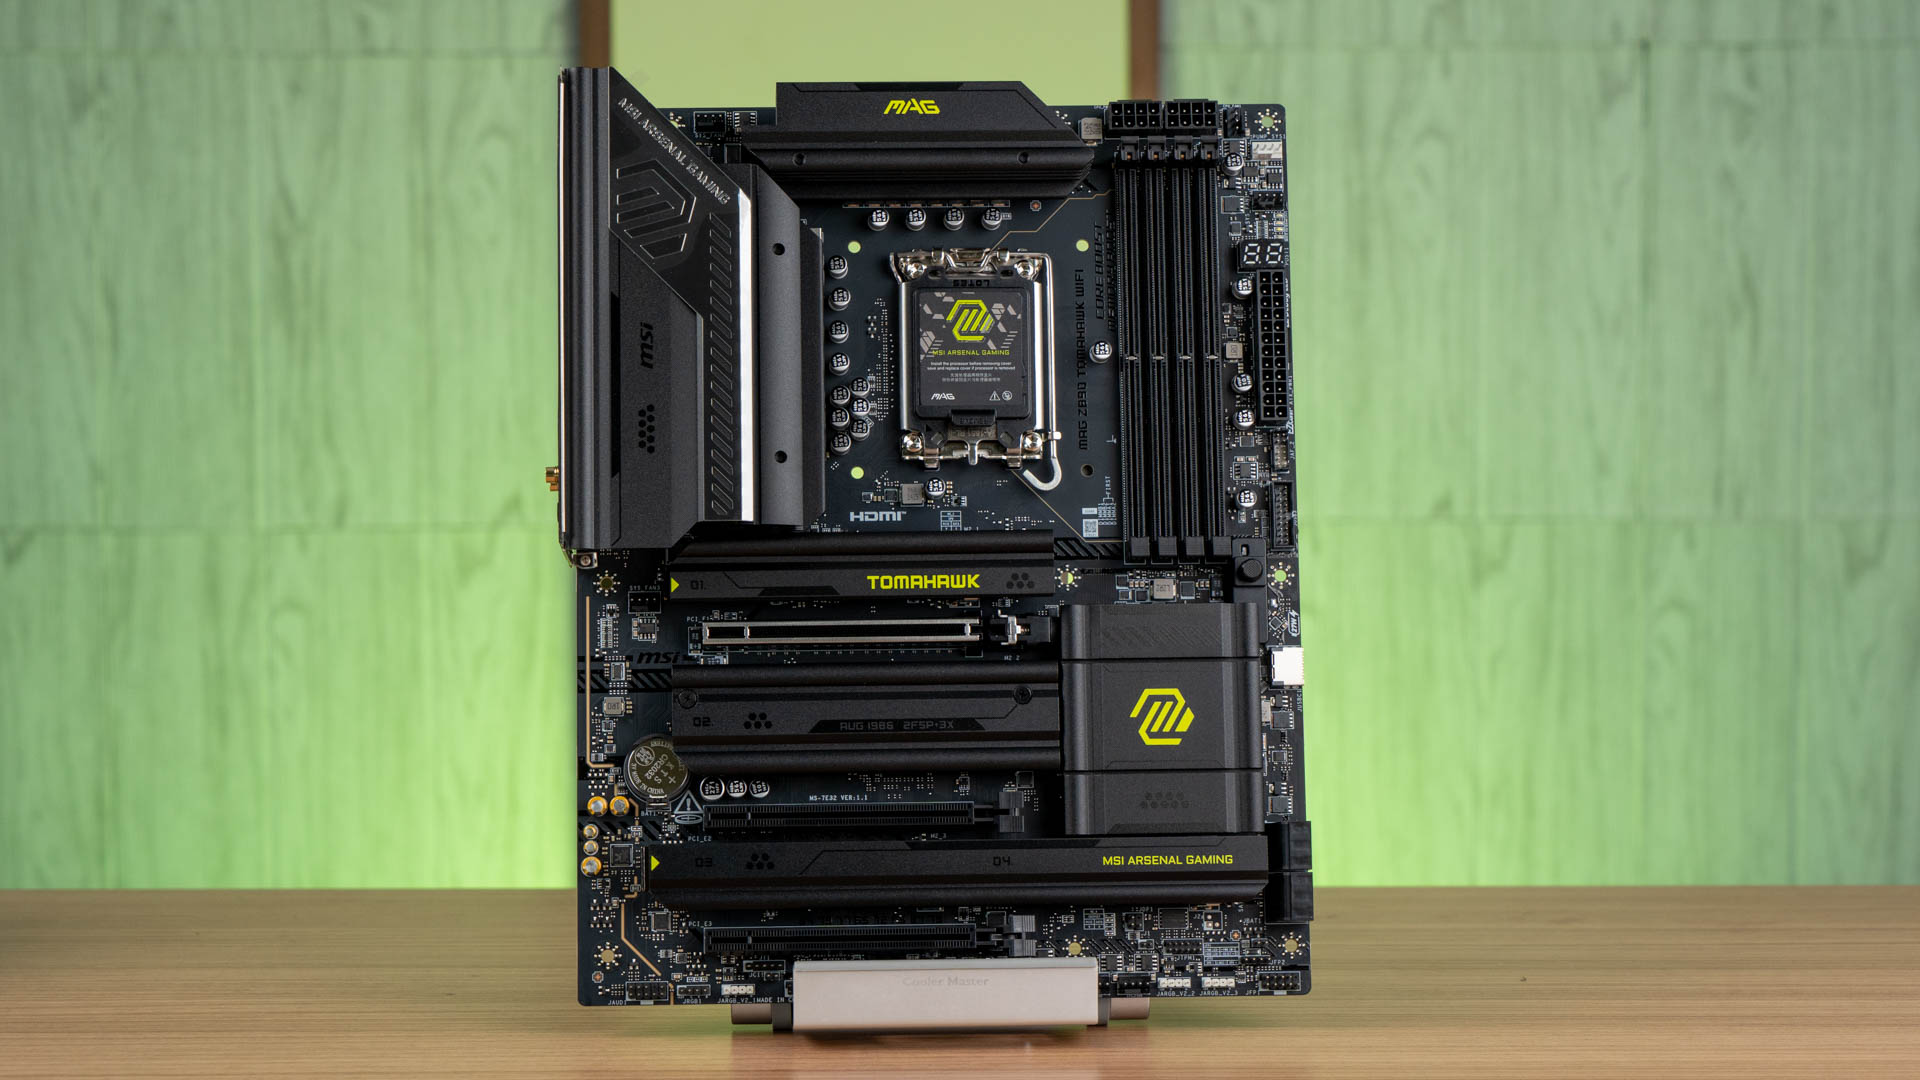
\includegraphics[scale=0.1]{imagenes/z890tomahawk.png}
  \caption{MSI MAG Z890 TOMAHAWK WIFI}
\end{figure}

Al seleccionar una tarjeta madre, es esencial considerar la compatibilidad con el procesador, el soporte para tecnologías actuales como PCIe 5.0 y DDR5, y las características específicas que se ajusten a tus necesidades, ya sea para gaming, trabajo profesional o uso general.
